\documentclass{article}
\usepackage{hyperref}
\usepackage{graphicx}

\title{Networking Concepts}
\author{}
\date{}

\begin{document}
\maketitle

\section*{Slides}
\href{files/networking-concepts/Fundamentals+of+Networking+for+Effective+Backends-v5.pdf}{Slides}

\section*{Standard communication models for Networking}

A standard model allows decoupling, so that the layers can be worked on or upgraded without worrying about the rest.

\subsection*{OSI (Open Systems Interconnect) Model}
\href{https://en.wikipedia.org/wiki/OSI_model}{OSI (Open Systems Interconnect) Model}

7 Layers each describe a specific networking component
\begin{itemize}
    \item Layer 7 - Application - HTTP/FTP/gRPC
    \item Layer 6 - Presentation - Encoding, Serialization
    \item Layer 5 - Session - Connection establishment, TLS
    \item Layer 4 - Transport - UDP/TCP
    \item Layer 3 - Network - IP
    \item Layer 2 - Data link - Frames, Mac address Ethernet
    \item Layer 1 - Physical - Electric signals, fiber or radio waves
\end{itemize}

\subsection*{The TCP/IP Model or Internet Protocol Suite}
\href{https://en.wikipedia.org/wiki/Internet_protocol_suite}{The TCP/IP Model or Internet Protocol Suite}

Much simpler than OSI, just 4 layers
\begin{itemize}
    \item Application (Layer 5, 6 and 7)
    \item Transport (Layer 4)
    \item Internet (Layer 3)
    \item Data link (Layer 2)
\end{itemize}
Physical layer is not officially covered in the model

\section*{Data Link Layer}

\subsection*{ARP (Address Resolution Protocol)}
It is used to translate IP addresses to MAC addresses, since IPs are changeable and MAC addresses are (usually) fixed. ARP is local.

\href{https://www.tcpdump.org/manpages/tcpdump.1.html}{\texttt{tcpdump}}

Tcpdump prints out a description of the contents of packets on a network interface.

\texttt{tcpdump -n -i wlp3s0 arp}

\texttt{tcpdump} with src and dst filters

\texttt{tcpdump -n -v -i wlp3s0 src 192.168.1.2 or dst 142.243.66.23}

To deliver the packet to the destination host, the source IP, destination IP, source MAC address, and destination MAC address should be known. Some basic rules for the packet flow:

\begin{itemize}
    \item If the destination host is present in the same network, then the packet is delivered directly to the destination host.
    \item If the destination host is present in a different network, then the packet is delivered to the default gateway first which in turn delivers the packet to the destination host.
    \item If ARP is not resolved then ARP will be resolved first.
    \item MAC address never crosses its broadcast domain.
\end{itemize}

\subsection*{Host to Host Communication}

Finding a device with a unique MAC address in a network is done by sending requests to all devices in the network. Only the device with the intended MAC address accepts the connection. But when the network is of a bigger scale than a simple home network, this method is not possible to scale. This is where IP addresses and routers come into play. Routers have two different IP addresses for the two networks they are connecting. When sending an IP packet (layer 3, router) there is a process of AND (\&)ing with the subnet mask to find out if the packet is destined to the same network or another, and passing forward until the TTL of the packet goes to zero or the destination is found.

\textbf{TTL - Time to Live} - this gives the count of how many hops a packet can survive. \textbf{TTL} is decreased by 1 every hop. TTL is needed because without it the packets might hop from router to router indefinitely.

\textit{Note [Optimization]} Keeping your server and database in the same subnet will be more efficient than those two being in separate subnets. Because the subnets are usually connected by a router (the routers live in both networks), if the router is congested, we are gonna see delays. Instead, we can use a switch in between the database and the backend.

\section*{Network Layer}

\href{https://en.wikipedia.org/wiki/Internet_Protocol}{IP} is the network layer communications protocol.

IP Addresses are a layer 3 property. Can be set automatically or statically, has \textit{network} and \textit{host} portions. 4 bytes in IPv4 - 32 bits.

\begin{itemize}
    \item a.b.c.d/x (a, b, c, d, x are integers). x is the network bits, remaining are the host. \href{https://en.wikipedia.org/wiki/Classless_Inter-Domain_Routing}{CIDR Notation}
\end{itemize}

\subsection*{ICMP (Internet Control Message Protocol)}
It is used by network devices, including routers, to send error messages and operational information indicating success or failure when communicating with another IP address. It is used by ping and traceroute.

\texttt{ping google.com}

\texttt{traceroute google.com}

\texttt{tcpdump -n -i wlp3s0 icmp}

\section*{Transport Layer}

\subsection*{\href{https://en.wikipedia.org/wiki/User_Datagram_Protocol}{UDP (User Datagram Protocol)}}

Layer 4 protocol, sits on top of the IP protocol (Network layer). While IP can address a host using IP addresses, UDP has the ability to address processes in a host using ports. Simpler and stateless protocol, compared to TCP. Has 8-byte header on top of 20 bytes of the IP packet. Used for:

\begin{itemize}
    \item Video Streaming
    \item VPN
    \item DNS
    \item WebRTC uses UDP. Websockets, on the other hand, use TCP
    \item Games
    \item P2P
\end{itemize}

Multiplexing (many to one) and demultiplexing (one to many). IP targets hosts only. Each host can have multiple applications running. Ports can be used to identify the 'apps' or 'processes'. The sender multiplexes all inputs into single IP packets into UDP, and the receiver demultiplexes UDP datagrams in IP packets to each app or process. A four-tuple (Source IP, Source Port, Destination IP, Destination Port) can represent every communication between two devices.

\textit{Note} Every time there is a mapping like in DNS, ARP tables, there's a chance of poisoning - ARP poisoning, DNS poisoning.

\textit{Note} Because we have 65535 ports, we can have a maximum of 65535 connections (theoretically) between a client IP and a single server process assuming the client uses all its ports to connect to the server process. Practically though, some of the ports are already reserved.

Capturing DNS server requests and responses using \texttt{tcpdump}:

\texttt{nslookup google.com 8.8.8.8}

\texttt{tcpdump -n -v -i wlp3s0 src 8.8.8.8 or dst 8.8.8.8}

\subsection*{\href{https://en.wikipedia.org/wiki/Transmission_Control_Protocol}{TCP (Transmission Control Protocol)}}

Similar to UDP, it's a Layer 4 protocol and can address processes in a host using ports. It 'controls' the transmission, unlike UDP which is like a firehose. Requires a connection before transmitting data. Connection is made using a 'handshake'. Hence it's stateful. Has 20 bytes header. Used for reliable communications like:

\begin{itemize}
    \item Remote Shell
    \item Database Connections
    \item Web Communications (HTTP1, HTTP2 is built on top of TCP, HTTP3 is built on top of QUIC which is built on top of UDP and aims to be better than TCP)
    \item Any bidirectional communication
\end{itemize}

TCP Connection is a Layer 5 (session) concept. The connection between client and server must be there to send data, can't send data outside of a connection, requires a 3-way TCP handshake.

The connection is identified by four properties (Source IP, Source Port, Destination IP, Destination Port). These four properties are combined and hashed and saved as a file descriptor (also called sockets).

\textit{Note} Socket often refers specifically to an internet socket or TCP socket. An internet socket is minimally characterized by the following:

\begin{itemize}
    \item local socket address, consisting of the local IP address and (for TCP and UDP, but not IP) a port number
    \item protocol: A transport protocol, e.g., TCP, UDP, raw IP. This means that (local or remote) endpoints with TCP port 53 and UDP port 53 are distinct sockets, while IP does not have ports.
    \item A socket that has been connected to another socket, e.g., during the establishment of a TCP connection, also has a remote socket address.
\end{itemize}

The Transmission Control Protocol differs in several key features compared to the User Datagram Protocol:

\begin{itemize}
    \item Ordered data transfer: the destination host rearranges segments according to a sequence number
    \item Retransmission of lost packets: any cumulative stream not acknowledged is retransmitted
    \item Error-free data transfer: corrupted packets are treated as lost and are retransmitted
    \item Flow control: limits the rate a sender transfers data to guarantee reliable delivery. The receiver continually hints the sender on how much data can be received (receiver sends an \texttt{ACK} with its window size[max 64KB but can be scaled up with the window scaling factor(0-14), so hat window size can go upto 1GB]). When the receiving host's buffer fills, the next acknowledgment suspends the transfer and allows the data in the buffer to be processed. Employs a \texttt{window sliding mechanism}.
    \item Congestion control: the receiver might handle the load but the middle boxes(routers) might not. lost packets (presumed due to congestion) trigger a reduction in data delivery rate
\end{itemize}

\subsubsection*{Maximum Segment Size}

\href{https://www.cloudflare.com/learning/network-layer/what-is-mss/}{MSS (maximum segment size)} limits the size of packets, or small chunks of data, that travel across a network. MSS measures the non-header portion of a packet, which is called the payload. MSS is determined by another metric that has to do with packet size: \href{https://www.cloudflare.com/learning/network-layer/what-is-mtu/}{MTU (maximum transmission unit)}, which does include the TCP and IP (Internet Protocol) headers.

Essentially, the MSS is equal to MTU minus the size of a TCP header and an IP header:

$$ MTU - (TCP header + IP header) = MSS $$

\begin{center}
    \begin{figure}[h]
        \centering
        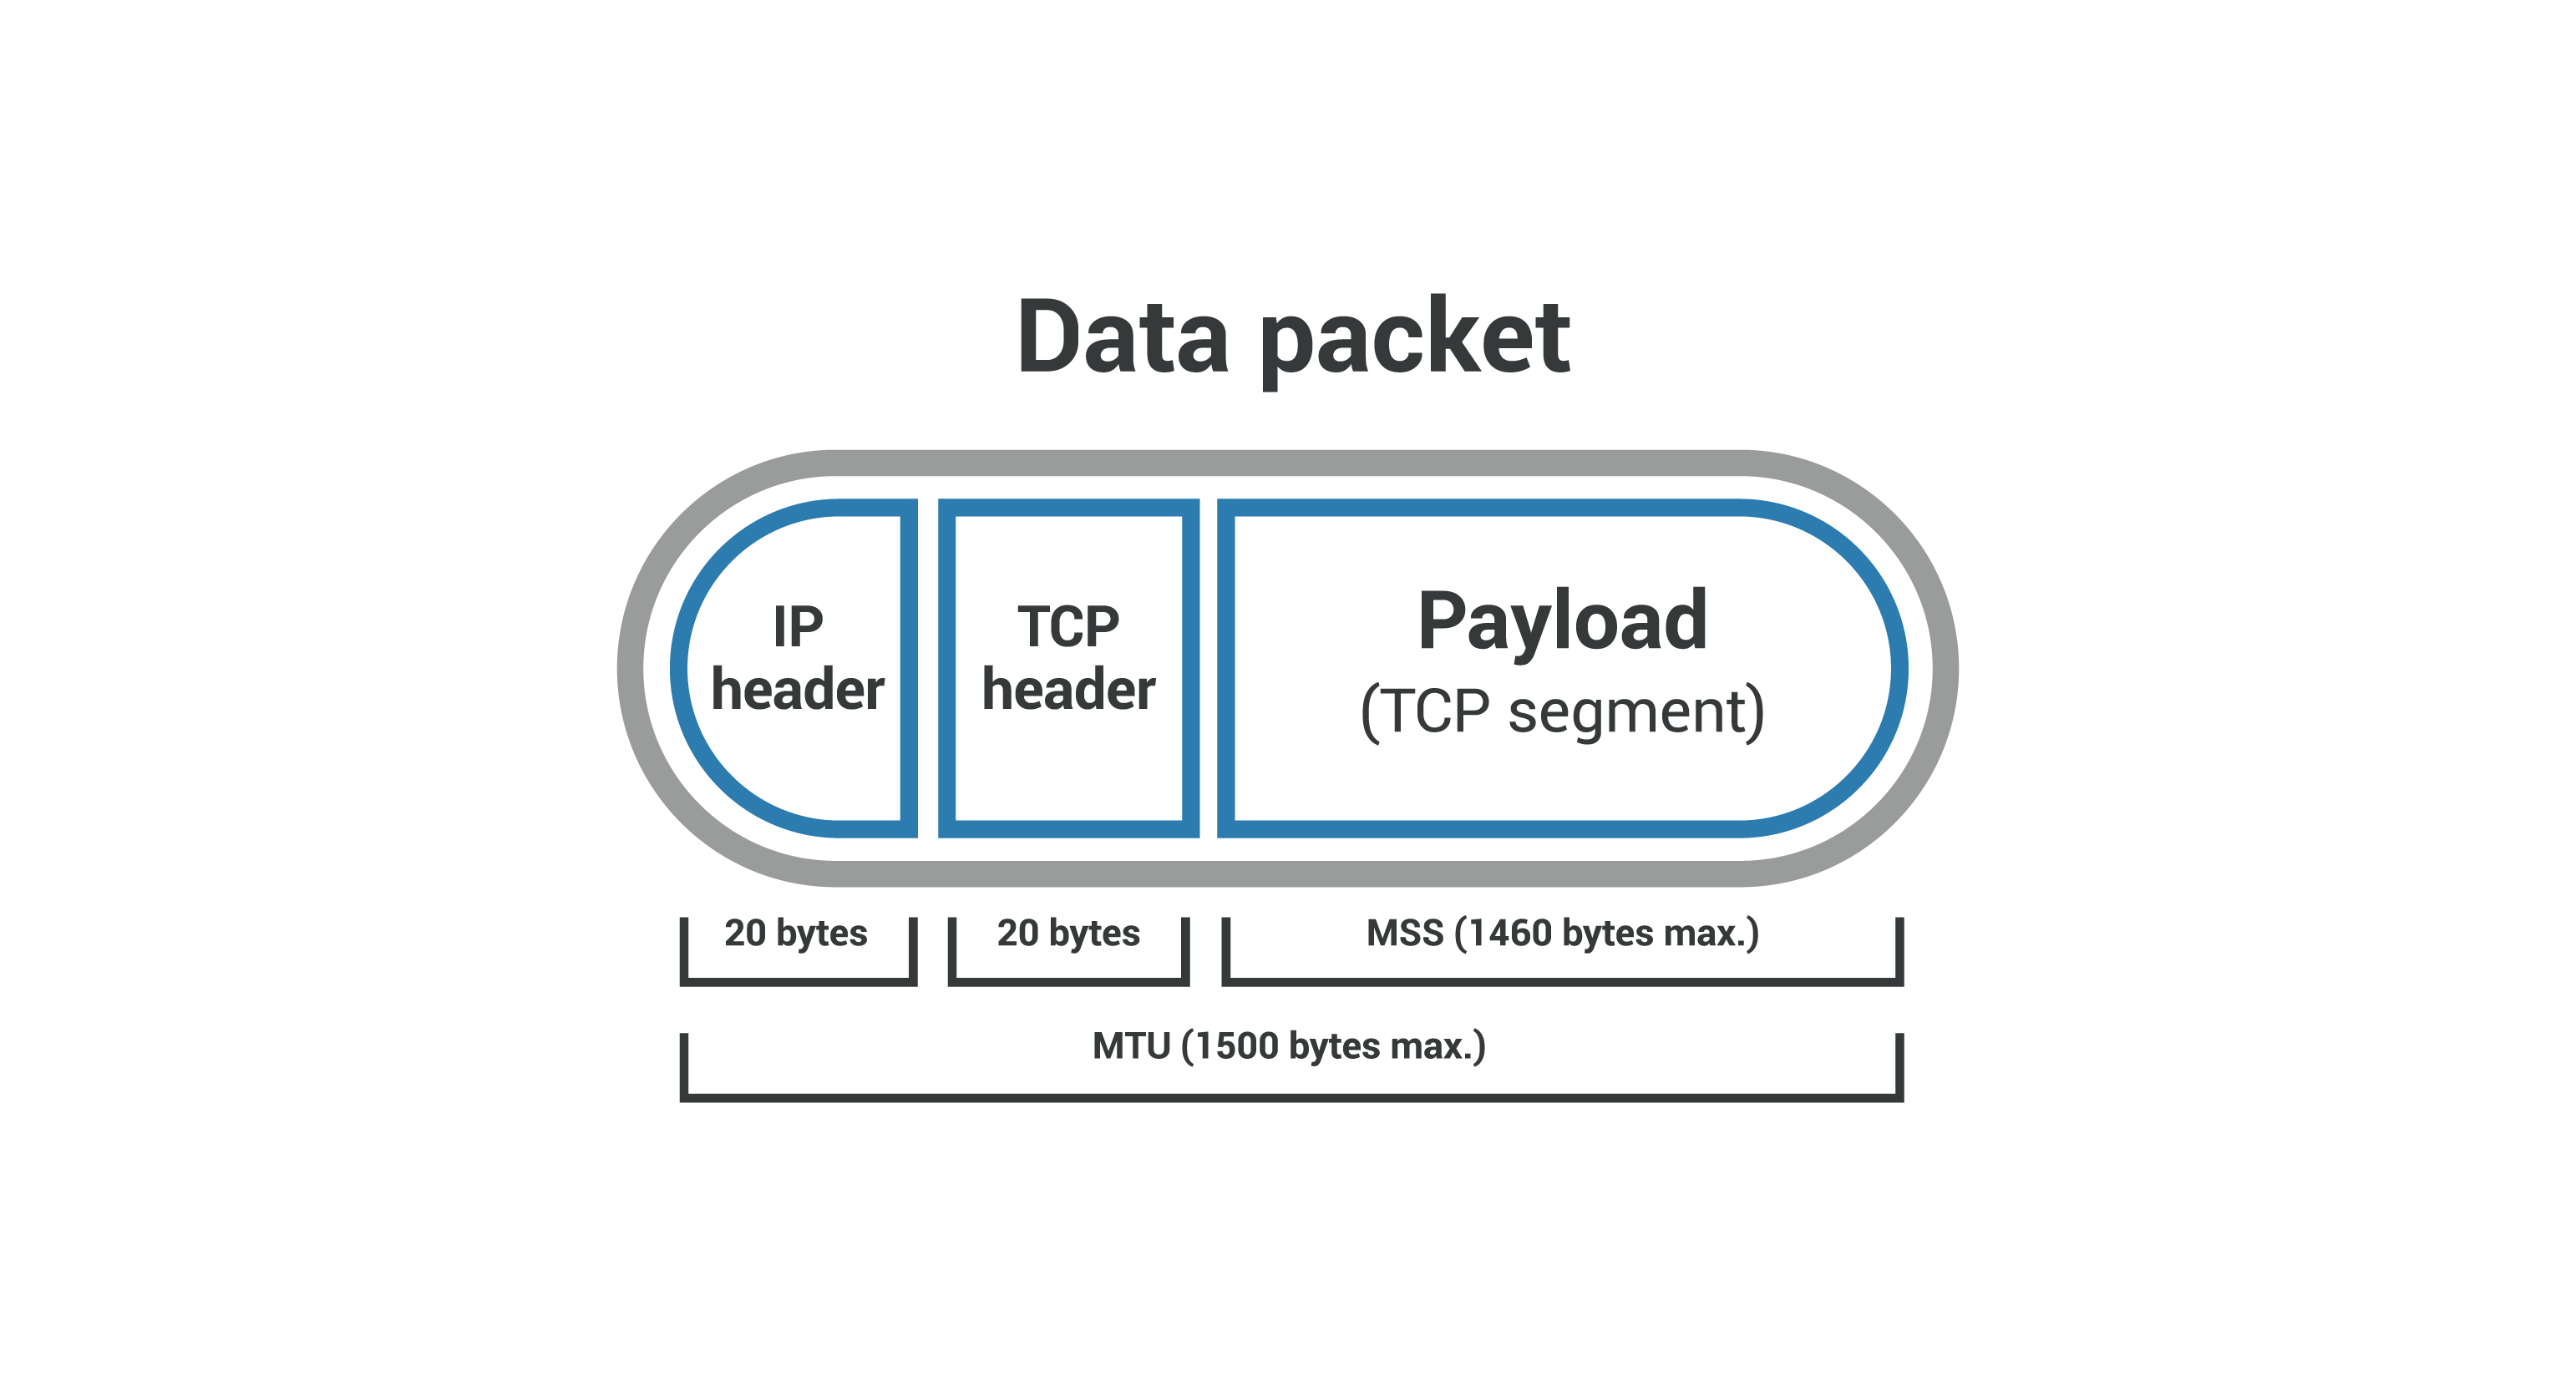
\includegraphics[width=0.6\linewidth]{files/networking-concepts/data-packet.png}
        \caption{A data packet}
    \end{figure}
\end{center}

One of the key differences between MTU and MSS is that if a packet exceeds a device's MTU, it is broken up into smaller pieces, or "fragmented." In contrast, if a packet exceeds the MSS, it is dropped and not delivered.

The maximum MTU of the internet is 1500 bytes, and the maximum MSS is 1460 bytes.

> Since then various other transmission systems have come and gone, but the lowest MTU value of them has still been Ethernet at 1500 bytes. Going bigger than the lowest MTU on a network will either result in IP fragmentation, or the need to do path MTU detection. Both of which have their own sets of problems. Even if sometimes large OS vendors dropped the default MTU to even lower at times.

\subsection*{NAT (Network Address Translation)}
IPV4 has a limit of 4 billion adressess which is not enough considering the number of devices connected to the Internet.IPV6 also solves this issue but for IPV4 adressing, NAT allows multiples of devices to  access the internet while also remaining private inside a network. It gives one public IP address(the gateway) and multiple private adresses for internal use. While it was inventeted to help with the ipv4 addressing issue, NAT also has a usecase for Layer 4 load balancing.

All devices have the same public IP address which is the router. The source port and IP adress is being mapped to a different source Port and IP for communication with the internet. This mapping called the 'NAT table' lives in the router has mappings to/from public and private ip-port pairs.

NAT uses the IP ranges - 192.168.x.x, 10.0.0.x allocated specifically for private networks.


\end{document}
